\chapter{Regression}
\label{ch:regression}

\textsuperscript{87}Rb is radioactive and decays to
\textsuperscript{87}Sr with a decay constant of
$\lambda=1.42\times{10}^{-5}$~Myr\textsuperscript{-1}.
\textsuperscript{86}Sr is a second isotope of Sr that does not have a
radioactive parent. Together these three nuclides form the basis of a
geochronometer:
\begin{equation}
  \left[\frac{{}^{87}Sr}{{}^{86}Sr}\right] =
  \left[\frac{{}^{87}Sr}{{}^{86}Sr}\right]_\circ +
  \left[\frac{{}^{87}Rb}{{}^{86}Sr}\right]
  \left(e^{\lambda{t}}-1\right)
  \label{eq:Rb-Sr}
\end{equation}

\noindent where $t$ is the age of the system, in millions of years,
and $[{}^{87}Sr/{}^{86}Sr]_\circ$ is the non-radiogenic
\textsuperscript{87}Sr/\textsuperscript{86}Sr ratio, i.e. the ratio
that was initially present in the sample at $t=0$. When applied to
multiple measurements, Equation~\ref{eq:Rb-Sr} fits the generic
formula for a straight line:
\begin{equation}
  y_i = \beta_0 + \beta_1~x_i
  \label{eq:y=a+bx}
\end{equation}

where $x_i$ and $y_i$ are the
\textsuperscript{87}Rb/\textsuperscript{86}Sr- and
\textsuperscript{87}Sr/\textsuperscript{86}Sr-ratios of the
$i$\textsuperscript{th} aliquot (out of $n$), respectively.
$x=\{x_1,\ldots,x_n\}$ is also known as the \textbf{independent
  variable} and $y=\{y_1,\ldots,y_n\}$ as the \textbf{dependent
  variable}. The following table shows an example of eight Rb--Sr
compositions from the same rock:

\begin{center}
  \begin{tabular}{c|cccccccc}
    $i$ & 1 & 2 & 3 & 4 & 5 & 6 & 7 & 8 \\ \hline
    $[{}^{87}Rb/{}^{86}Sr] = x_i$ & 2.90 & 7.14 & 9.10 &
    3.41 & 1.91 & 7.15 & 5.92 & 8.28 \\
    $[{}^{87}Sr/{}^{86}Sr] = y_i$ & 0.745 & 0.803 & 0.823 & 0.737 &
    0.720 & 0.793 & 0.789 & 0.807
  \end{tabular}
  \captionof{table}{Rb--Sr composition of eight aliquots
    ($1\leq{i}\leq{8}$) of the same sample.}
  \label{tab:Rb-Sr}
\end{center}

Visualising the data on a scatter plot:

\noindent\begin{minipage}[t][][b]{.3\textwidth}
  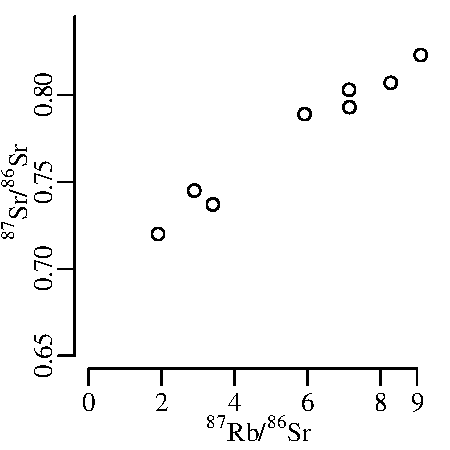
\includegraphics[width=\textwidth]{../figures/RbSr.pdf}\\
\end{minipage}
\begin{minipage}[t][][t]{.7\textwidth}
  \captionof{figure}{Isochron plot for the Rb--Sr data.  The scatter
    plot of eight \textsuperscript{87}Rb/\textsuperscript{86}Sr- and
    \textsuperscript{87}Sr/\textsuperscript{86}Sr-ratios forms an
    array of points along a line whose intercept marks the initial
    \textsuperscript{87}Sr/\textsuperscript{86}Sr-composition, and
    whose slope is a function of the age ($t =
    \ln[1+\beta_1]/\lambda$). The linear trend is not perfect due to
    analytical uncertainty, which has dispersed the data.  }
  \label{fig:Rb-Sr}
\end{minipage}

The dispersion of the data around the straight line can be captured by
a slightly modified version of Equation~\ref{eq:y=a+bx}:
\begin{equation}
  y_i = \beta_0 + \beta_1~x_i + \epsilon_i
  \label{eq:y=a+bx+e}
\end{equation}

\noindent where $\epsilon_i$ is the \textbf{residual} noise around the
best fit line which, in this situation, is attributed to the dependent
variable only.\\

The linear trend seems quite strong in the Rb--Sr example, but this
may not always be the case. The \textbf{correlation coefficient} is a
parameter that can be used to quantify the strength and test the
significance of an apparent linear trend.

\section{The correlation coefficient}
\label{sec:corrcoef}

Recall the definition of \emph{standard deviation} ($\sigma_x,
\sigma_y$) and \emph{covariance} ($\sigma_{x,y}$) from
Section~\ref{sec:normalproperties}. Then Pearson's correlation
coefficient is defined as:
\begin{equation}
  \rho = \frac{\sigma_{x,y}}{\sigma_x\sigma_y}
  \label{eq:rho}
\end{equation}

Section~\ref{sec:normalparameters} showed that $\sigma_x, \sigma_y$
and $\sigma_{x,y}$ are unknown but can be \emph{estimated} from the
data using Equations~\ref{eq:stdevrepeat} and \ref{eq:sxy}:
\begin{equation*}
  \begin{split}
  s[x] & = \sqrt{\sum\limits_{i=1}^{n}\frac{1}{n-1}(x_i-\bar{x})^2} \\
  s[x,y] & = \sum\limits_{i=1}^{n}\frac{1}{n-1}(x_i-\bar{x})(y_i-\bar{y})
  \end{split}
\end{equation*}

\noindent where $\bar{x}$ and $\bar{y}$ are the arithmetic means of
$x$ and $y$, respectively. Then Pearson's correlation coefficient
\emph{for samples} is defined as:
\begin{equation}
  r = \frac{s[x,y]}{s[x]s[y]}
  \label{eq:r}
\end{equation}

Both $\rho$ and $r$ take on values between $-1$ and $+1$. It is also
common for the degree of correlation to be quantified as $r^2$, which
produces values between 0 and 1. $r^2$ is also known as the
\textbf{coefficient of determination}.

\noindent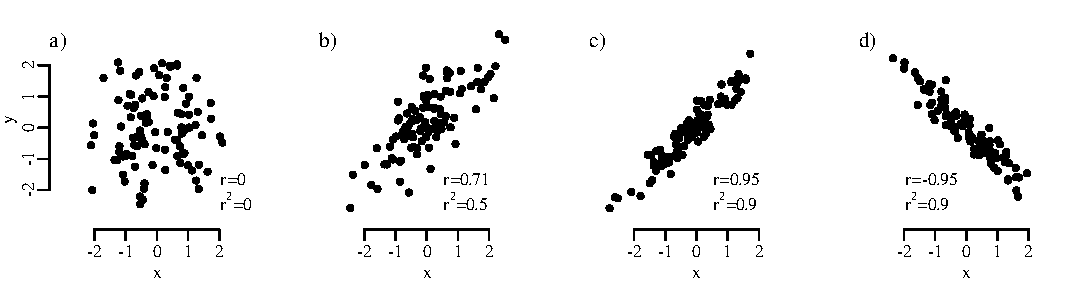
\includegraphics[width=\textwidth]{../figures/r.pdf} \begingroup
\captionof{figure}{Four synthetic bivariate normal datasets exhibiting
  different degrees of correlation between the x- and
  y-variable. Panel a) displays no correlation, b) a weak positive
  correlation, c) a strong positive correlation, and d) a strong
  negative correlation.\\}
\label{fig:r}
\endgroup

The `weak' and `strong' qualifiers in Figure~\ref{fig:r} are
subjective assessments of the linear trend. A more objective
evaluation is possible by the fact that
\begin{equation}
  t = \frac{r\sqrt{n-2}}{\sqrt{1-r^2}}
  \label{eq:tr}
\end{equation}

\noindent follows a t-distribution with $n-2$ degrees of freedom. Thus
we can formally test whether the apparent correlation between the
\textsuperscript{87}Sr/\textsuperscript{86}Sr- and
\textsuperscript{87}Rb/\textsuperscript{86}Sr-ratios in
Figure~\ref{fig:Rb-Sr} is statistically significant. Plugging the data
of Table~\ref{tab:Rb-Sr} into Equation~\ref{eq:r} yields a correlation
coefficient of $r = 0.985$.  This seems high enough but let's subject
it to a hypothesis test anyway:

\begin{enumerate}
\item Formulate two hypotheses:

  \noindent\begin{minipage}{.4\textwidth}
  $H_0$ (\textbf{null hypothesis})
  
  \vspace{1em}
  
  $H_{\!A}$ (\textbf{alternative hypothesis}):
\end{minipage}
\begin{minipage}{.2\textwidth}
\end{minipage}
\begin{minipage}{.2\textwidth}
  $\rho=0$
  
  \vspace{1em}
  
  $\rho\neq{0}$
\end{minipage}
\begin{minipage}{.2\textwidth}
\end{minipage}\\

\item Plugging $r = 0.985$ into Equation~\ref{eq:tr} yields a test
  statistic of

  \[
  t = \frac{0.985\sqrt{8-2}}{\sqrt{1-0.985^2}} = 13.98
  \]

\item Tabulating some key quantiles for $t$ under $H_0$:
  
  \begin{center}
    \begin{tabular}{c|c@{\gap}c@{\gap}c@{\gap}c@{\gap}
        c@{\gap}c@{\gap}c@{\gap}c@{\gap}c@{\gap}c@{\gap}c@{\gap}c}
      $t$ & -3.14 & -2.45 & -1.94 & -1.44 & -0.72 &
      0 & 0.72 & 1.44 & 1.94 & 2.45 & 3.14 & \emph{13.98}\\
      $P(t<T)$ & 0.01 & 0.025 & 0.05 & 0.1 & 0.25 &
      0.5 & 0.75 & 0.9 & 0.95 & 0.975 & 0.99 & \emph{0.9999958}\\
      $P(t>T)$ & 0.99 & 0.975 & 0.95 & 0.9 & 0.75 & 0.5 &
      0.25 & 0.1 & 0.05 & 0.025 & 0.010 & \emph{0.0000042}
    \end{tabular}
  \end{center}

  \noindent where the observed value is marked in italics.
  
\item We will use a confidence level $\alpha = 0.05$.

\item Marking the two-sided rejection region in bold:
  
  \begin{center}
    \begin{tabular}{c|c@{\gap}c@{\gap}c@{\gap}c@{\gap}
        c@{\gap}c@{\gap}c@{\gap}c@{\gap}c@{\gap}c@{\gap}c@{\gap}c}
      $t$ & \textbf{-3.14} & \textbf{-2.45} & -1.94 & -1.44 & -0.72 &
      0 & 0.72 & 1.44 & 1.94 & \textbf{2.44} &
      \textbf{3.14} & \textbf{\emph{13.98}}\\
      $P(t<T)$ & \textbf{0.01} & \textbf{0.025} & 0.05 & 0.1 & 0.25 &
      0.5 & 0.75 & 0.9 & 0.95 & 0.975 & 0.99 & \emph{0.9999958}\\
      $P(t>T)$ & 0.99 & 0.975 & 0.95 & 0.9 & 0.75 & 0.5 &
      0.25 & 0.1 & 0.05 & \textbf{0.025} & \textbf{0.010} &
      \textbf{\emph{0.0000042}}
    \end{tabular}
  \end{center}

  The rejection region consists of all $|t|>{2.40}$.

\item The observed value of $t=13.98$ clearly falls inside the
  rejection region, so $H_0$ is rejected.
  
\end{enumerate}

\noindent\begin{minipage}[t][][b]{.6\textwidth}
  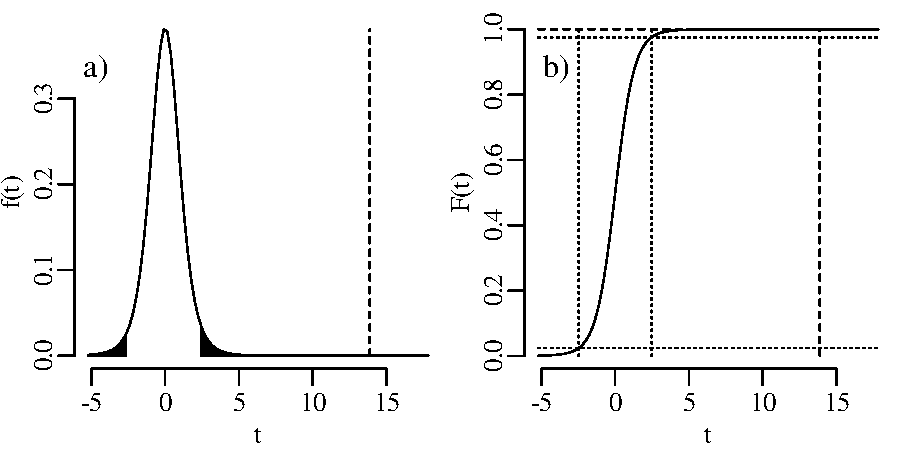
\includegraphics[width=\textwidth]{../figures/tr.pdf}\\
\end{minipage}
\begin{minipage}[t][][t]{.4\textwidth}
  \captionof{figure}{a) PDF and b) CDF of a t-distribution with 6
    degrees of freedom. The two-sided rejection region (for $\alpha =
    0.05$) is marked in black. The vertical dashed line marks the
    observed value of t = 13.98 and plots inside the rejection
    region. Therefore the test rejects the null hypothesis that
    $\rho=0$, leading to the conclusion that the data are
    significantly correlated.}
  \label{fig:tr}
\end{minipage}

Now that we have convinced ourselves that the correlation is
significant, we can try to fit a line through the data. In order to
find the best possible fit, we first need to define what we need with
`best'. There are many ways to do this, but the most common of these
is the method of least squares.

\section{Least Squares}
\label{sec:leastsquares}

As the name suggests, the least squares criterion quantifies the
misfit of the line through the data as the sum of the squared
residuals:
\begin{equation}
ss \equiv \sum_{i=1}^{n} \epsilon_i^2 = \sum_{i=1}^{n} (y_i - \beta_0 - \beta_1 x_i)^2
\label{eq:ss}
\end{equation}

Let us take a wild guess and assume that $\beta_0=0.6$ and
$\beta_1=0.03$:

\begin{center}
  \begin{tabular}{c|cccccccc}
    $i$ & 1 & 2 & 3 & 4 & 5 & 6 & 7 & 8 \\ \hline
    $x_i$ & 2.90 & 7.14 & 9.10 & 3.41 & 1.91 & 7.15 & 5.92 & 8.28 \\
    $y_i$ & 0.745 & 0.803 & 0.823 & 0.737 & 0.720 & 0.793 & 0.789 & 0.807 \\ \hline
    $\beta_0 + \beta_1 x_i$ & 0.687 & 0.8142 & 0.873 & 0.7023 &
    0.6573 & 0.8145 & 0.7776 & 0.8484 \\
    $\epsilon_i$ & 0.058 & -0.0112 & -0.05 & 0.0347 & 0.0627 &
    -0.0215 & 0.0114 & -0.0414
  \end{tabular}
  \captionof{table}{The same data as Table~\ref{tab:Rb-Sr}. $y_i$ are
    the observed and $\beta_0 + \beta_1 x_i$ the \emph{fitted} values
    of the dependent variable. The residuals $\epsilon_i$ are the
    differences between these two sets of numbers.}
\end{center}

Plugging the $\epsilon_i$-values into Equation~\ref{eq:ss} yields a
sum of squares $ss=0.013$. Evaluating some other values:\medskip

\noindent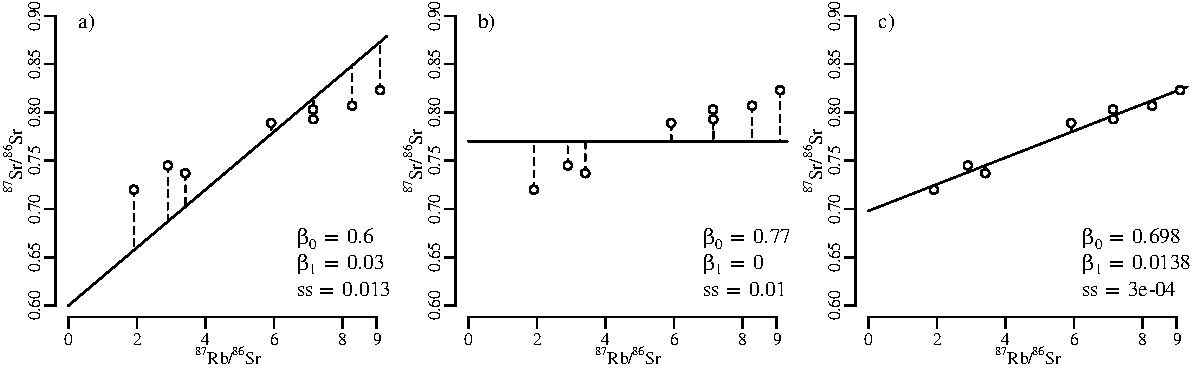
\includegraphics[width=\textwidth]{../figures/tryRbSr.pdf}
\begingroup \captionof{figure}{Three guesses for the intercept
  ($\beta_0$) and slope ($\beta_1$) of the Rb--Sr isochron data of
  Figure~\ref{fig:Rb-Sr}.  Dashed lines mark the residuals. The lines
  in panels a) and b) are too steep and too shallow,
  respectively. Consequently, the sums of their squared residuals
  ($ss$) are relatively large. Panel c) shows a better fit and a
  smaller sum of squares.\medskip} \endgroup

Instead of minimising $ss$ by iterating over all possible values of
$\beta_0$ and $\beta_1$, we can also find the optimal solution
directly by taking the partial derivatives of Equation~\ref{eq:ss}
w.r.t. $\beta_0$ and $\beta_1$ and setting them to zero:
\begin{equation}
\begin{cases}
    \frac{\partial ss}{\partial\beta_0} = 2 \sum(y_i - \beta_0 - \beta_1 x_i) = 0\\
    \frac{\partial ss}{\partial\beta_1} = 2 \sum(y_i - \beta_0 - \beta_1 x_i) x_i = 0
\end{cases}
\end{equation}

By solving this system of equations, it can be shown that:
\begin{equation}
\begin{cases}
  \hat{\beta}_0 = \left(\sum x_i^2 \sum y_i - \sum x_i \sum x_iy_i\right) /
  \left(n \sum x_i^2 - \left(\sum x_i\right)^2\right)\\
  \hat{\beta}_1 = \left(n\sum x_iy_i - \sum x_i \sum y_i \right) /
  \left(n \sum x_i^2 - \left(\sum x_i\right)^2\right)
\end{cases}
\label{eq:fitab}
\end{equation}

For the Rb--Sr data:

\begin{center}
  \begin{tabular}{c|cccccccc|c}
    $i$ & 1 & 2 & 3 & 4 & 5 & 6 & 7 & 8 & $\sum_{i=1}^{8}$ \\ \hline
    $x_i$ & 2.90 & 7.14 & 9.10 & 3.41 & 1.91 & 7.15 & 5.92 & 8.28 & 45.81 \\
    $y_i$ & 0.745 & 0.803 & 0.823 & 0.737 & 0.720 &
    0.793 & 0.789 & 0.807 & 6.217\\ \hline
    $x_i^2$ & 8.41 & 50.98 & 82.81 & 11.63 & 3.648 &
    51.12 & 35.05 & 68.56 & 312.2 \\
    $x_iy_i$ & 2.160 & 5.733 & 7.489 & 2.513 & 1.375 &
    5.670 & 4.671 & 6.682 & 36.29
  \end{tabular}
\end{center}

\noindent so that
\begin{equation*}
\begin{cases}
  \hat{\beta}_0 = \left(312.2 \times 6.217 - 45.81 \times 36.29 \right) /
  \left(8 \times 312.2 - 45.81^2\right) = 0.698 \\
  \hat{\beta}_1 = \left( 8 \times 36.29 - 45.81 \times 6.217 \right) /
  \left(8 \times 312.2 - 45.81^2\right) = 0.0138
\end{cases}
\end{equation*}

\section{Maximum Likelihood}
\label{sec:MLregression}

Least squares regression is one way to determine the fit parameters of
a straight line.  The method of maximum likelihood
(Sections~\ref{sec:binompar}, \ref{sec:poispar},
\ref{sec:normalparameters} and \ref{sec:FisherInformation}) is
another. This section will show that these two approaches produce
exactly the same results. Recall the general formulation of the linear
regression problem (Equation~\ref{eq:y=a+bx+e}):
\begin{equation*}
  y_i = \beta_0 + \beta_1~x_i + \epsilon_i
\end{equation*}

Let us assume that the residuals ($\epsilon_i$) are normally
distributed \emph{with zero mean}:
\begin{equation}
  f(\epsilon_i|\beta_0,\beta_1,\sigma) = \frac{1}{\sigma\sqrt{2\pi}}
  \exp\!\left[-\frac{\epsilon_i^2}{2\sigma^2}\right] \mbox{,~where~}
  \epsilon_i = \beta_0 + \beta_1 x_i - y_i
  \label{eq:normalresid}
\end{equation}

In that case, we can estimate $\beta_0$ and $\beta_1$ by maximising
the (log-)likelihood, in exactly the same fashion as the maximum
likelihood estimation algorithm of Section~\ref{sec:normalparameters}
and Equation~\ref{eq:Lnorm}
\begin{equation}
  \mathcal{L}(\beta_0,\beta_1,\sigma|\{x_1,y_1\},\ldots,\{x_n,y_n\}) =
  \prod\limits_{i=1}^{n}\frac{1}{\sigma\sqrt{2\pi}}
  \exp\!\left[-\frac{\epsilon_i^2}{2\sigma^2}\right]
  \label{eq:Lregression}
\end{equation}

Minimising Equation \ref{eq:ss} is equivalent to maximising Equation
\ref{eq:Lregression}:
\begin{equation}
\begin{split}
\underset{\beta_0,\beta_1}{\max}\left[\prod_{i=1}^n \mathcal{L}\right] = &
\underset{\beta_0,\beta_1}{\max}\left[\sum_{i=1}^n \ln\mathcal{L}\right] =
\underset{\beta_0,\beta_1}{\max}\left[\ln\!\left(\frac{1}{\sigma\sqrt{2\pi}}\right)-\sum_{i=1}^n\left(\frac{\epsilon_i^2}{2\sigma^2}\right)\right] \\
= & \underset{\beta_0,\beta_1}{\max}\left[-\sum_{i=1}^n\epsilon_i^2\right] = 
\underset{\beta_0,\beta_1}{\min}\left[\sum_{i=1}^{n} \epsilon_i^2\right] = \underset{\beta_0,\beta_1}{\min}(ss)
\end{split}
\end{equation}

This means that the least squares and maximum likelihood methods
produce exactly the same result, and that linear regression works best
when the residuals are normally distributed. Error propagation of the
estimated regression coefficients ($\hat{\beta}_0$, $\hat{\beta}_1$)
proceeds as in Section~\ref{sec:FisherInformation}:
\begin{equation}
  \begin{split}
    \Sigma_{\hat{\beta}} & = 
  \left[
    \begin{array}{@{}cc@{}}
      s[\hat{\beta}_0]^2 & s[\hat{\beta}_0,\hat{\beta}_1] \\
      s[\hat{\beta}_0,\hat{\beta}_1] & s[\hat{\beta}_1]^2 \\
    \end{array}
    \right] = 
  -\mathcal{H}^{-1} \\
  & =
    -\left[
      \begin{array}{@{}cc@{}}
        \frac{\partial^2{\mathcal{LL}}}{\partial{\beta_0^2}} &
        \frac{\partial^2{\mathcal{LL}}}{\partial{\beta_0}\partial{\beta_1}} \\
        \frac{\partial^2{\mathcal{LL}}}{\partial{\beta_0}\partial{\beta_1}} &
        \frac{\partial^2{\mathcal{LL}}}{\partial{\beta_1^2}}
      \end{array}
      \right]^{-1} \\
    & = -\left(\frac{1}{\sigma^2}
    \left[
      \begin{array}{@{}cc@{}}
        n & \sum_{i=1}^{n}x_i \\
        \sum_{i=1}^{n}x_i & \sum_{i=1}^{n}x_i^2
      \end{array}
      \right]\right)^{-1} \\
    & =
    \frac{\sigma^2}{\sum_{i=1}^{n}(x_i^2-\bar{x}^2)}
    \left[
      \begin{array}{@{}cc@{}}
        \sum_{i=1}^{n}x_i^2/n & -\bar{x} \\
        -\bar{x} & 1
      \end{array}
      \right]
  \end{split}
  \label{eq:sigmabeta}
\end{equation}

Equation~\ref{eq:sigmabeta} uses the standard deviation of the data
around the linear fit ($\sigma$). This parameter is generally unknown
and must be estimated from the data:
\begin{equation}
  \hat{\sigma} = \sqrt{\sum\limits_{i=1}^{n}
    \frac{(\hat{\beta}_0+\hat{\beta}_1x_i-y_i)^2}{n-2}}
  \label{eq:sigmahatregression}
\end{equation}

Equation~\ref{eq:sigmahatregression} looks similar to the usual
definition of the standard deviation (Equation~\ref{eq:stdevrepeat})
except that 2 degrees of freedom have been subtracted instead of 1,
because two parameters were estimated ($\hat{\beta}_0$ and
$\hat{\beta}_1$) instead of one ($\bar{x}$).\\

Equation~\ref{eq:sigmabeta} can be used to construct a
\textbf{confidence interval} for the regression coefficients. The
procedure for doing this is analogous to the construction of
confidence intervals around the mean (Equation~\ref{eq:tci}):
\begin{equation}
  \beta_0 \in \left\{\hat{\beta}_0 \pm t_{df,\alpha/2}~s[\hat{\beta}_0]\right\}
  \mbox{~and~}
  \beta_1 \in \left\{\hat{\beta}_1 \pm t_{df,\alpha/2}~s[\hat{\beta}_1]\right\}
  \label{eq:ciregression}
\end{equation}

\noindent where $df=n-2$. We can then construct a \textbf{confidence
  envelope} around the best fit line by observing that
$y=\beta_0+\beta_1x$ matches the equation for a sum, and applying the
corresponding error propagation formula (Equation~\ref{eq:addition}):
\begin{equation}
  y \in \left\{\hat{\beta}_0 + \hat{\beta}_1 x \pm t_{df,\alpha/2}
  \sqrt{s[\hat{\beta}_0]^2 + s[\hat{\beta}_1]^2 x^2 +
    2 s[\hat{\beta}_0,\hat{\beta}_1]x} \right\}
  \label{eq:envelope}
\end{equation}

Applying Equation~\ref{eq:envelope} to the Rb--Sr data and evaluating
$y$ for the full range of $x$-values:

\noindent\begin{minipage}[t][][b]{.33\textwidth}
  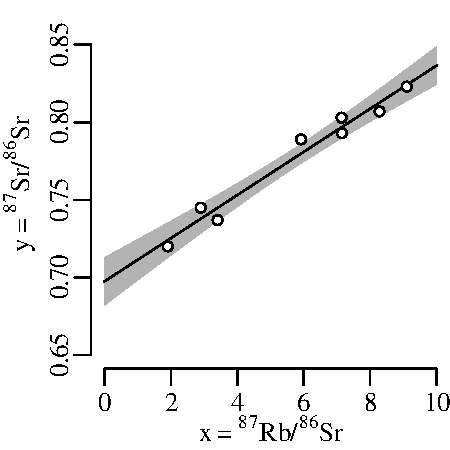
\includegraphics[width=\textwidth]{../figures/envelope.pdf}\\
\end{minipage}
\begin{minipage}[t][][t]{.67\textwidth}
  \captionof{figure}{The grey area represents a 95\% confidence
    envelope for the least squares regression of the Rb--Sr data. The
    curvature of this envelope reflects the increased uncertainty that
    is caused by \textbf{extrapolating} the data. The width of the
    confidence envelope is the smallest near the average of the
    measurements ($\bar{x}$, $\bar{y}$) and increases indefinitely
    beyond that.}
  \label{fig:envelope}
\end{minipage}

Recall that the standard error of the mean decreases with increasing
sample size (Section~\ref{sec:stderr}). Exactly the same phenomenon
applies to the standard errors of the regression parameters
(Equation~\ref{eq:sigmabeta}) and, hence, to the width of the
confidence envelope. In order to assess the likely range of
\emph{future outcomes}, the confidence envelopes produced by
Equation~\ref{eq:envelope} need to be enlarged to produce a
\textbf{prediction interval}:
\begin{equation}
  y \in \left\{\hat{\beta}_0 + \hat{\beta}_1 x \pm t_{df,\alpha/2}
  \sqrt{\hat{\sigma}^2 + s[\hat{\beta}_0]^2 + s[\hat{\beta}_1]^2 x^2 +
    2 s[\hat{\beta}_0,\hat{\beta}_1]x} \right\}
  \label{eq:prediction-interval}
\end{equation}

\noindent where $\hat{\sigma}$ is given by
Equation~\ref{eq:sigmahatregression}. Comparing confidence intervals
and prediction intervals for different sample sizes of three synthetic
datasets:

\noindent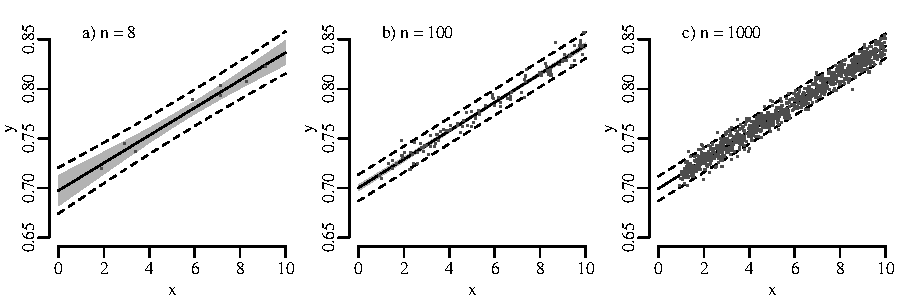
\includegraphics[width=\textwidth]{../figures/prediction-interval.pdf}
\begingroup \captionof{figure}{Confidence envelopes (grey) and
  prediction intervals (dashed lines) for three synthetic datasets of
  increasing size. Whereas the width of the confidence interval
  approaches zero for large datasets, the width of the prediction
  interval only decreases slightly.  }
\label{fig:prediction-interval}
\endgroup

\section{Common mistakes}
\label{sec:regression-caveats}

Three mistakes are commonly made in regression analysis:

\begin{enumerate}
\item{\bf p-hacking}: This problem was already discussed in
  section~\ref{sec:multipletesting} but bears repeating in the context
  of linear regression. When presented with a multivariate dataset
  (e.g. the concentration of $n$ chemical species in $m$ samples), it
  is common practice in exploratory data analysis to plot all pairs of
  variables against each other in an $n\times{m}$ grid of scatter
  plots. When doing this it is inevitable that some of these pairs
  exhibit a statistically significant correlation.

\noindent\begin{minipage}[t][][b]{\linewidth}
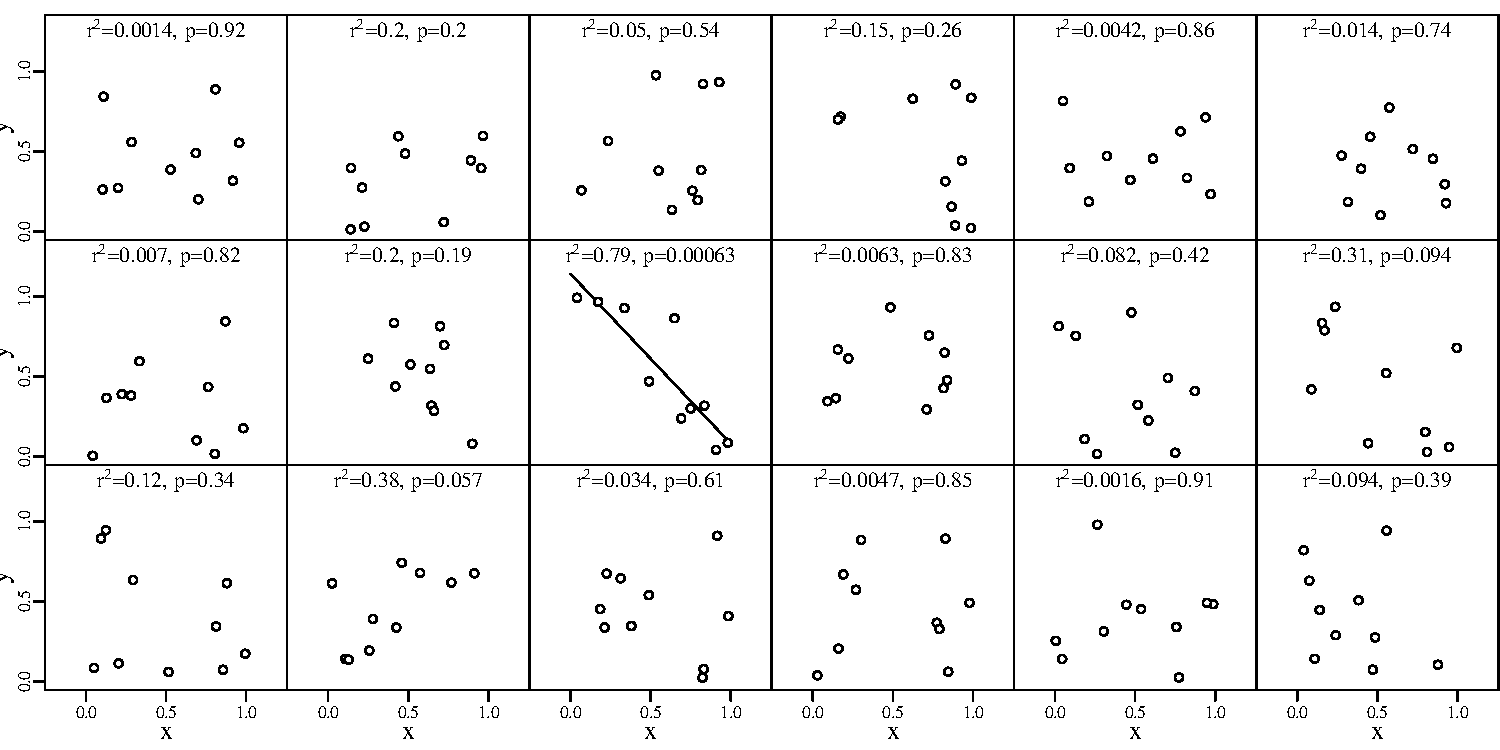
\includegraphics[width=\textwidth]{../figures/regression-p-hacking.pdf}
\captionof{figure}{18 scatter plots of bivariate random uniform data,
  with indication of the coefficient of determination ($r^2$) and the
  p-value for correlation. The one `significant' result (p-value =
  0.00063) is a Type-I error.}
  \label{fig:regression-p-hacking}
\end{minipage}

\item{\bf outliers}: High values for the correlation coefficient ($r$)
  and coefficient of determination ($r^2$) are often taken as evidence
  for correlation. However, these statistics are sensitive to extreme
  values.  A single outlier can have a disproportionally large effect,
  suggesting a significant correlation where there is none.

\noindent\begin{minipage}[t][][b]{.3\linewidth}
  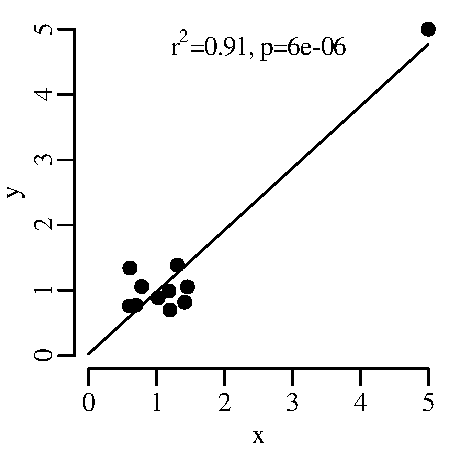
\includegraphics[width=\textwidth]{../figures/regression-outlier.pdf}
\end{minipage}
\begin{minipage}[t][][t]{.7\linewidth}
  \captionof{figure}{A synthetic dataset of ten clustered points
    around $\{x=1,y=1\}$ plus one outlier at $\{x=5,y=5\}$.  The
    cluster consists of the same values as the first panel of
    Figure~\ref{fig:regression-p-hacking}. But whereas the latter
    dataset was characterised by a coefficient of determination of
    almost zero ($r^2=0.0014$), the new dataset has a coefficient of
    determination that is close to one ($r^2=0.9$). Such is the
    disproportionate effect of the additional data point.  }
  \label{fig:regression-outlier}
\end{minipage}

\item{\bf Spurious correlation}: Let $x$, $y$ and $z$ be three
  \emph{independent} random datasets of 50 numbers.  Then the
  bivariate scatter plots of $y$ vs. $x$, $z$ vs. $x$ and $z$ vs. $y$
  do not exhibit any discernable correlation. However, plotting $y/z$
  vs. $x/z$, or $z$ vs. $x/z$ produces strong correlations:

\noindent\begin{minipage}[t][][b]{\linewidth}
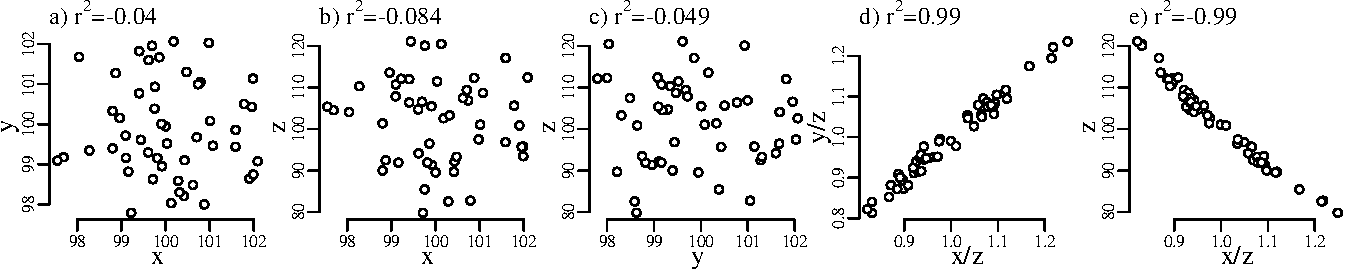
\includegraphics[width=\textwidth]{../figures/spurious.pdf}
\captionof{figure}{a--c) Three random datasets of 50 points each,
  drawn from normal distributions with means $\mu_x=\mu_y=\mu_z=100$
  and standard deviations $\sigma_x=\sigma_y=1$ and $\sigma_z=10$,
  respectively. The three datasets are independent, so
  $\rho_{x,y}=\rho_{x,z}=\rho_{y,z}=0$. However, the ratio of $x/z$ is
  strongly correlated with d) $y/z$, and with e) $z$. This correlation
  is entirely spurious and has no scientific value.\\}
  \label{fig:spurious}
\end{minipage}

The data clouds in panels d) and e) of Figure~\ref{fig:spurious} are
strongly correlated even though $x$, $y$, $z$ are uncorrelated.  This
correlation arises because $z$ appears in both axes.  This phenomenon
was first described by Karl Pearson\footnote{Pearson, K.,
1897. Mathematical contributions to the theory of evolution.—on a form
of spurious correlation which may arise when indices are used in the
measurement of organs. Proceedings of the Royal Society of London,
60(359--367), pp.489--498.} of the eponymous correlation coefficient
($r$, Equation~\ref{eq:r}), who also showed that it is possible to
predict the expected correlation coefficient (or `null correlation')
associated with the spurious effect. In the general case of four
samples $w$, $x$, $y$ and $z$, the \textbf{ratio correlation} of $w/y$
and $x/z$ is given by:
\begin{equation}
  \noindent \rho_{\frac{w}{y},\frac{x}{z}} \approx
  \frac{\rho_{w,x}\left[\frac{\sigma_w}{\mu_w}\right]
    \left[\frac{\sigma_x}{\mu_x}\right] -
    \rho_{w,z}\left[\frac{\sigma_w}{\mu_w}\right]
    \left[\frac{\sigma_z}{\mu_z}\right] -
    \rho_{x,y}\left[\frac{\sigma_x}{\mu_x}\right]
    \left[\frac{\sigma_y}{\mu_y}\right] +
    \rho_{y,z}\left[\frac{\sigma_y}{\mu_y}\right]
    \left[\frac{\sigma_z}{\mu_z}\right]
  }{
    \sqrt{\left[\frac{\sigma_w}{\mu_w}\right]^2 +
      \left[\frac{\sigma_y}{\mu_y}\right]^2 -
      2 \rho_{w,y}\left[\frac{\sigma_w}{\mu_w}\right]
      \left[\frac{\sigma_y}{\mu_y}\right]}
    \sqrt{\left[\frac{\sigma_x}{\mu_x}\right]^2 +
      \left[\frac{\sigma_z}{\mu_z}\right]^2 -
      2 \rho_{x,z}\left[\frac{\sigma_x}{\mu_x}\right]
      \left[\frac{\sigma_z}{\mu_z}\right]
    }
  }
  \label{eq:spurious}
\end{equation}

Substituting $z$ for $y$ and $y$ for $w$ in
Equation~\ref{eq:spurious}, and considering that $\rho_{z,z}=1$, we
can show that:
\begin{equation}
  \noindent \rho_{\frac{y}{z},\frac{x}{z}} \approx
  \frac{\rho_{y,x}\left[\frac{\sigma_y}{\mu_y}\right]
    \left[\frac{\sigma_x}{\mu_x}\right] -
    \rho_{y,z}\left[\frac{\sigma_y}{\mu_y}\right]
    \left[\frac{\sigma_z}{\mu_z}\right] -
    \rho_{x,z}\left[\frac{\sigma_x}{\mu_x}\right]
    \left[\frac{\sigma_z}{\mu_z}\right] +
    \left[\frac{\sigma_z}{\mu_z}\right]^2
  }{
    \sqrt{\left[\frac{\sigma_y}{\mu_y}\right]^2 +
      \left[\frac{\sigma_z}{\mu_z}\right]^2 -
      2 \rho_{y,z}\left[\frac{\sigma_y}{\mu_y}\right]
      \left[\frac{\sigma_z}{\mu_z}\right]}
    \sqrt{\left[\frac{\sigma_x}{\mu_x}\right]^2 +
      \left[\frac{\sigma_z}{\mu_z}\right]^2 -
      2 \rho_{x,z}\left[\frac{\sigma_x}{\mu_x}\right]
      \left[\frac{\sigma_z}{\mu_z}\right]
    }
  }
  \label{eq:spuriousxzyz}
\end{equation}

Similarly, substituting $w$ for $z$, and setting $y=1$ and
$\sigma_y=0$ in Equation~\ref{eq:spurious}:
\begin{equation}
  \noindent \rho_{z,\frac{x}{z}} \approx
  \frac{\rho_{z,x}\left[\frac{\sigma_z}{\mu_z}\right]
    \left[\frac{\sigma_x}{\mu_x}\right] -
    \left[\frac{\sigma_z}{\mu_z}\right]^2
  }{
    \left[\frac{\sigma_z}{\mu_z}\right]
    \sqrt{\left[\frac{\sigma_x}{\mu_x}\right]^2 +
      \left[\frac{\sigma_z}{\mu_z}\right]^2 -
      2 \rho_{x,z}\left[\frac{\sigma_x}{\mu_x}\right]
      \left[\frac{\sigma_z}{\mu_z}\right]
    }
  }
  \label{eq:spuriouszxz}
\end{equation}

For the example of Figure~\ref{fig:spurious}, where
$\rho_{x,y}=\rho_{x,z}=\rho_{y,z}=0$, the expected \textbf{null
  correlation} for $x/z$ and $y/z$ is obtained from
Equation~\ref{eq:spuriousxzyz}:
\begin{equation}
  \noindent \rho_{\frac{y}{z},\frac{x}{z}} \approx
  \frac{
    \left[\frac{\sigma_z}{\mu_z}\right]^2
  }{
    \sqrt{\left[\frac{\sigma_y}{\mu_y}\right]^2 +
      \left[\frac{\sigma_z}{\mu_z}\right]^2}
    \sqrt{\left[\frac{\sigma_x}{\mu_x}\right]^2 +
      \left[\frac{\sigma_z}{\mu_z}\right]^2}
  }
  =
  \frac{
    \left[\frac{10}{100}\right]^2
  }{
    \left[\frac{1}{100}\right]^2 +
      \left[\frac{10}{100}\right]^2
  }
  = 0.990
  \label{eq:spuriousxzyzindepxyz}
\end{equation}

\noindent which is in excellent agreement with the observed
correlation coefficient of Figure~\ref{fig:spurious}d. Similarly, the
null correlation for $x/z$ and $z$ is obtained from
Equation~\ref{eq:spuriouszxz}:
\begin{equation*}
  \noindent \rho_{z,\frac{x}{z}} \approx
  \frac{
    - \left[\frac{10}{100}\right]^2
  }{
    \left[\frac{10}{100}\right]
    \sqrt{\left[\frac{1}{100}\right]^2 +
      \left[\frac{10}{100}\right]^2
    }
  } = -0.995
\end{equation*}

\noindent which explains the strong negative correlation in
Figure~\ref{fig:spurious}e.  It is important to be aware of the ratio
correlation phenomenon because scatter plots of ratios are commonplace
in geology. Two examples are the
\textsuperscript{87}Rb/\textsuperscript{86}Sr --
\textsuperscript{87}Sr/\textsuperscript{86}Sr isochron plot from the
beginning of this chapter, and the Zr--Zr/Y tectonic discrimination
diagram of igneous geochemistry.
 
\end{enumerate}

\section{Weighted regression}
\label{sec:weightedregression}

The least squares regression algorithm of
Sections~\ref{sec:leastsquares} and \ref{sec:MLregression} assumed
that the residuals ($\epsilon_i$ in Equation~\ref{eq:y=a+bx+e})
followed a normal distribution with zero mean and equal standard
deviation. Using statistical jargon, we assumed that the data are
\emph{homoscedastic}. However, real datasets are often
\textbf{heteroscedastic}, i.e. their standard deviation varies between
aliquots.\\

Consider, for example, the case of (Rb--Sr) isochron regression.  It
is based on \textsuperscript{87}Rb/\textsuperscript{86}Sr and
\textsuperscript{87}Sr/\textsuperscript{86}Sr isotope measurements
that are obtained by mass spectrometry. The uncertainties of these
measurements are known and may vary significantly between
aliquots. Due to the spurious correlation issue of
Section~\ref{sec:regression-caveats}.3, these uncertainties may also
be correlated. To illustrate the effect of these complications,
consider a simple three-point example:

\begin{center}
\begin{tabular}{c|cc|ccccc}
  $i$ & $X$ & $Y$ & $x$ & $s[x]$ & $y$ & $s[y]$ & $s[x,y]$ \\
  \hline
  1 & 10 & 20 & 10.5 & 1 & 20.5 & 1 & 0.9 \\
  2 & 20 & 30 & 19.5 & 1 & 29.9 & 1 & 0.9 \\
  3 & 30 & 40 & 25.1 & 3 & 45.2 & 5 & -13.5
\end{tabular}
\captionof{table}{Synthetic three-aliquot dataset. $X$ and $Y$ the
  \emph{true} values; $x$ and $y$ are three \emph{measurements},
  $s[x]$ and $s[y]$ their respective standard errors, and $s[x,y]$
  their covariance. The uncertainties differ between the three
  samples, which are therefore heteroscedastic.}
\label{tab:york}
\end{center}

The uncertainties can be visualised as \textbf{error ellipses} (see
Figures~\ref{fig:norm2dmarginal} and \ref{fig:cov}):

\noindent\begin{minipage}[t][][b]{.35\textwidth}
  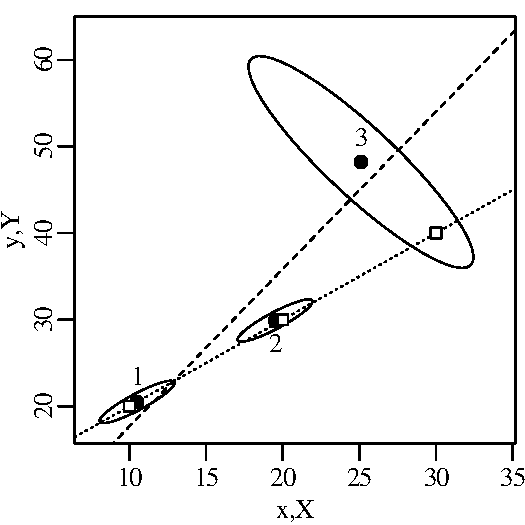
\includegraphics[width=\textwidth]{../figures/errorfit.pdf}
\end{minipage}
\begin{minipage}[t][][t]{.65\textwidth}
  \captionof{figure}{Synthetic data of Table~\ref{tab:york}. The white
    squares are the true population values ($X$ and $Y$) of three
    aliquots. The black squares are three measurements ($x$ and
    $y$). The ellipses represent 95\% confidence regions for bivariate
    normal distributions with means $x$ and $y$, and (co)variances
    $s[x]^2$, $s[y]^2$ and $s[x,y]$. The true values fall on a line
    with intercept $\beta_0=10$ and slope $\beta_1=1$ (dotted line).
    The unweighted least squares fit (dashed line) has an intercept of
    $\beta_0=1.9$ and slope $\beta_1=1.63$. This poor result is
    entirely due to the third data point, whose disproportionally
    large uncertainties are not properly accounted for by the ordinary
    least squares regression algorithm.  }
  \label{fig:errorfit}
\end{minipage}

To account for the unequal uncertainties of the three aliquots, we
need to replace the likelihood function of the unweighted regression
algorithm (Equation~\ref{eq:Lregression}):
\begin{equation*}
  \mathcal{L}(\beta_0,\beta_1,\sigma|x_1,y_1,\ldots,x_n,y_n) =
  \prod\limits_{i=1}^{n}\frac{1}{\sigma\sqrt{2\pi}}
  \exp\!\left[-\frac{(y_i - \beta_0 - \beta_1 x_i)^2}{2\sigma^2}\right]
\end{equation*}

\noindent with a different function that is based on the bivariate
normal distribution (Equation~\ref{eq:2dgauss}):
\begin{equation}
  \begin{split}
  & \mathcal{L}_w(\beta_0,\beta_1,\boldsymbol{x}_1,\ldots,\boldsymbol{x}_n|x_1,y_1,\ldots,x_n,y_n) =  \\
  & \prod\limits_{i=1}^{n}\frac{1}{2 \pi \sqrt{|\Sigma_i|}}
  \exp\!\left(-\frac{1}{2}
  \left[
    \begin{array}{@{}c@{}}
      x_i - \boldsymbol{x}_i\\
      y_i - \beta_0 - \beta_1\boldsymbol{x}_i\\
    \end{array}
    \right]^T
  \Sigma_i^{-1}
  \left[
  \begin{array}{@{}c@{}}
      x_i - \boldsymbol{x}_i\\
      y_i - \beta_0 - \beta_1\boldsymbol{x}_i\\
    \end{array}
  \right] \right) \\
  \end{split}
  \label{eq:york}
\end{equation}

\noindent where $\boldsymbol{x}_1,\ldots,\boldsymbol{x}_n$ are the
\emph{fitted} values for the independent variable $x$. This is the
most likely value for $X$ given the measurement $x$ and the analytical
uncertainties. The $\boldsymbol{x}$-values must be estimated from the
data along with the intercept ($\beta_0$) and slope ($\beta_1$) of the
regression model. Equation~\ref{eq:york} can be maximised numerically.

\noindent\begin{minipage}[t][][b]{.65\textwidth}
  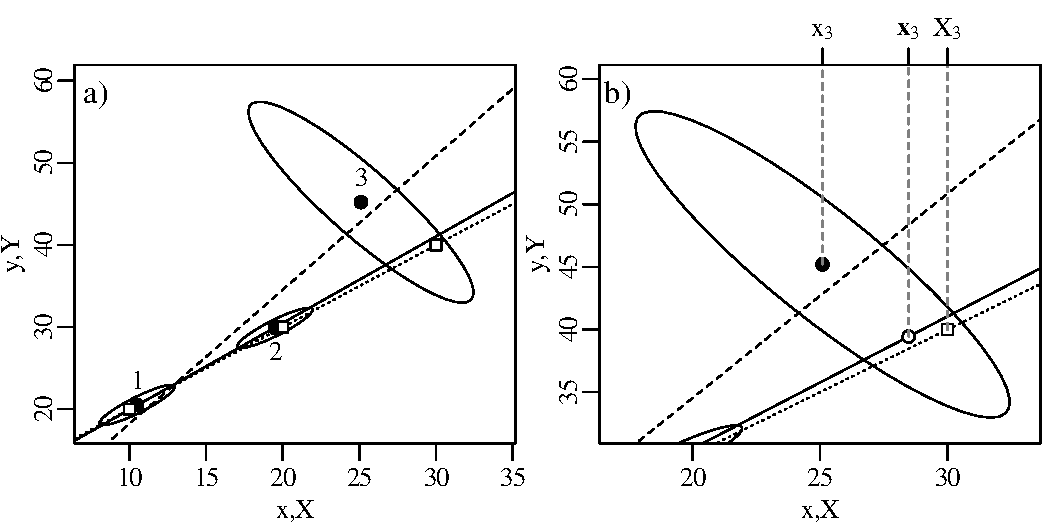
\includegraphics[width=\textwidth]{../figures/yorkfit.pdf}
\end{minipage}
\begin{minipage}[t][][t]{.35\textwidth}
  \captionof{figure}{a) the same as Figure~\ref{fig:errorfit}, but
    with the weighted regression result added as a solid line. Its
    intercept is $\beta_0=9.4$ and its slope is $\beta_1=1.05$. These
    values are much closer to the true values (dotted line) than the
    ordinary least squares solution (dashed line) is. b) Zooming into
    aliquot~3 shows the true value of the independent variable
    ($X_3$), its measured value ($x_3$), and the fitted value
    $\boldsymbol{x}_3$.  }
  \label{fig:yorkfit}
\end{minipage}
